\documentclass[conference]{IEEEtran}

\IEEEoverridecommandlockouts
\usepackage{cite}
\usepackage{amsmath,amssymb,amsfonts}
\usepackage{algorithmic}
\usepackage{graphicx}
\usepackage{textcomp}
\usepackage{xcolor}
\usepackage{fancyhdr}
\usepackage{lipsum}

\def\BibTeX{{\rm B\kern-.05em{\sc i\kern-.025em b}\kern-.08em
    T\kern-.1667em\lower.7ex\hbox{E}\kern-.125emX}}
    
\fancypagestyle{firstpagefooter}{%
  \fancyhf{}
  \renewcommand\headrulewidth{0pt}
  \fancyfoot[R]{Sporadic Server, Hamm-Lippstadt Hochschule}
}

\pagestyle{empty}

\begin{document}
\title{Sporadic Server}

\author{\IEEEauthorblockN{Vytaras Juraska}
\IEEEauthorblockB{\textit{Electronics Engineering (6\textsuperscript{th} Semester)} \\
\textit{Hamm-Lippstadt Hochschule}\\
Lippstadt, Germany \\
vytaras.juraska@stud.hshl.de}
}

\maketitle

\begin{abstract}
an explanation and a deep dive on the working concept, the history of development and the usage of a very specific solution to aperiodic and unpredictable task scheduling - Sporadic Server. Understanding and analyzing the relevancy and connection when applying specified scheduling server to the current time and age technology standards.
\end{abstract}


%\begin{IEEEkeywords}
%component, formatting, style, styling, insert
%\end{IEEEkeywords}

\thispagestyle{firstpagefooter}

\section{Introduction}
There are many ways of scheduling a task, since typically a task is periodic, predictable, has a lot of properties, which help managing priorities of scheduling and understanding the required steps to manage tasks with limited computational power and other resources. But what would happen, if our task would lose a lot of properties, which provide predictability? Well, Sporadic Server approach is a unique solution to this unique problem.

\subsection{Sporadic/Aperiodic Tasks}

Sporadic/Aperiodic Tasks - a completely unknown and unpredictable task: arrival times are unknown, execution times might be also unknown. To understand what kind of solution should be applied we should understand the worst case scenario of this specific task, since if we can handle the worst, we can handle any type of aperiodic task. So the characteristics of a hardest to schedule aperiodic task are:

\begin{itemize}
    \item Minimum time between arrivals of each task, high frequency.
    \item Having a known deadline, which would have the highest priority, the requirement of running the task until completion.
\end{itemize}

\textbf{NOTE} Further on compare the characteristics of the periodic and aperiodic tasks. What variables we know, and which exact ones we don't know/can't predict? (Figure \ref{tasks})

\begin{figure}[htbp]
\centerline{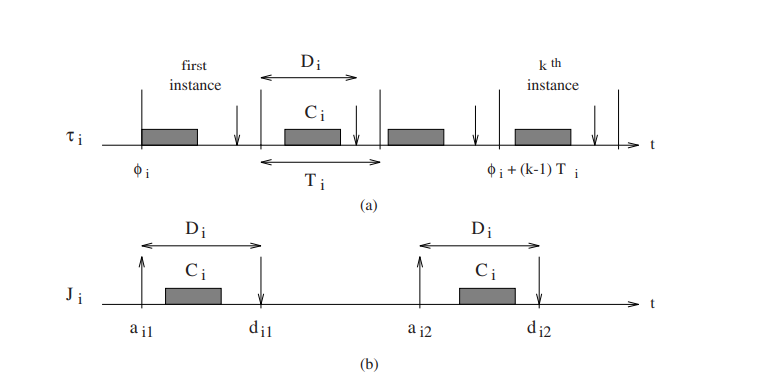
\includegraphics[scale=.5]{Tasks.png}}
\caption{Sequences of Periodic Tasks (a) and Aperiodic Tasks (b)}
\label{tasks}
\end{figure}

\subsection{Implementing Standard Solutions}
What would happen, what would be the result, if we would use standard solutions to manage these specific types of tasks, is it effective, where do the standard solutions succeed and where do they fail.

\subsection{Sporadic Server}
Sporadic Server - an implementation on how to handle and store Sporadic Tasks.
Definition of sporadic server and theoretical working concept.

\textbf{NOTE} Example of a Sporadic server working principle, when aperiodic tasks are considered to be a Medium-Priority (Figure \ref{example1}).

\begin{figure}[htbp]
\centerline{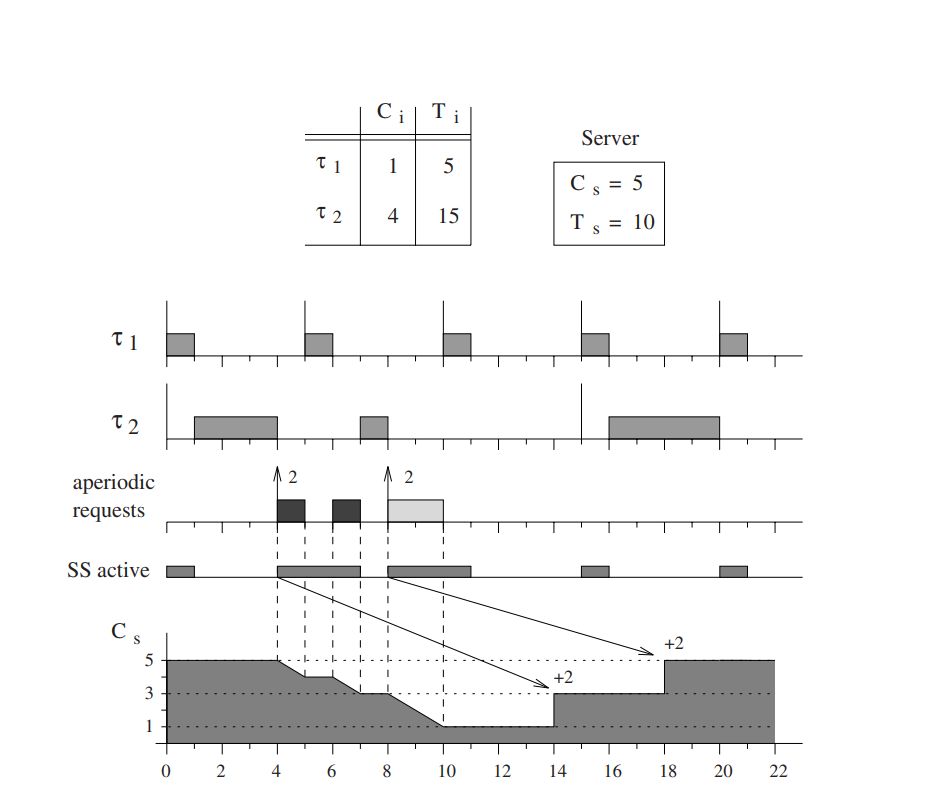
\includegraphics[scale=.38]{Example1.png}}
\caption{Medium-Priority Sporadic Server}
\label{example1}
\end{figure}

\textbf{NOTE} Example of a Sporadic server working principle, when aperiodic tasks are considered to be a High-Priority (Figure \ref{example2}).

\begin{figure}[htbp]
\centerline{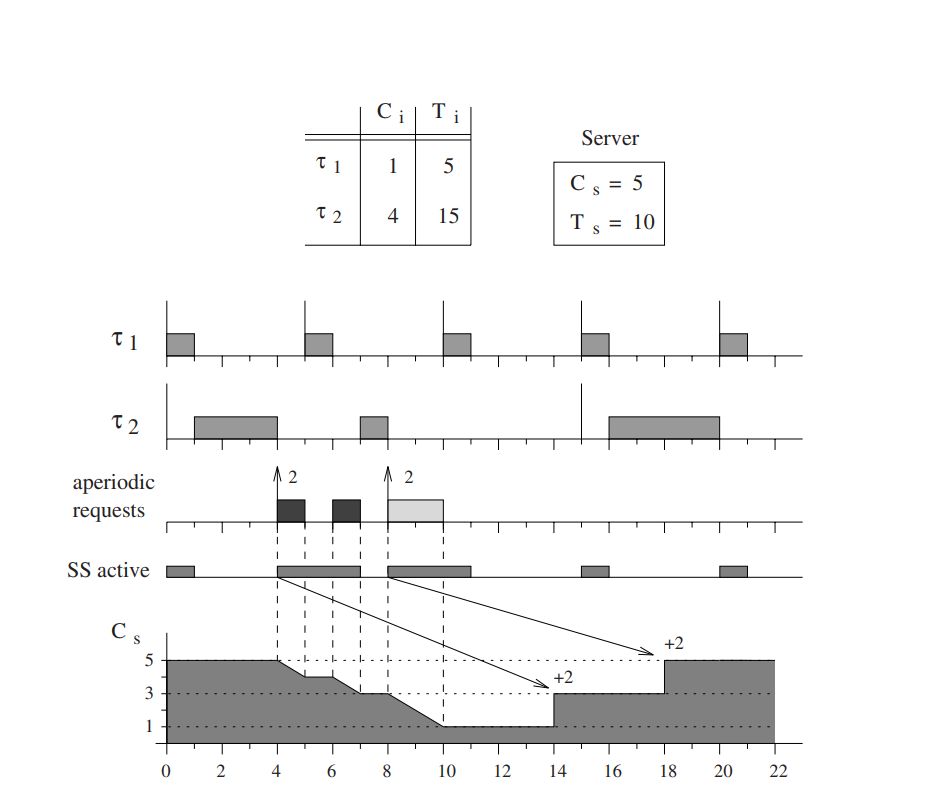
\includegraphics[scale=.39]{Example1.png}}
\caption{High-Priority Sporadic Server}
\label{example2}
\end{figure}

\section{Implementation}
An example of how could this be implemented. Implementation in  Ada [3]

\section{History of Development}
A detailed timeline of how this method came to be developed, who developed it and what were the intentions

\section{Usage and Appliance}
Where is it applied in real situations, where is it used in

\section{Advantages}
Any positive advantages related to this method, why and where is it useful to use this method

\section{Disadvantages}
Any disadvantages, which might lead to certain issues, why and where this method can not be applied

\section{Evaluation}
Personal opinion, is it useful, is there future for this method?

\section{Conclusion}
Final thoughts, concluding the topic

\begin{thebibliography}{00}
\bibitem{b1} G. C. Buttazzo "Hard Real-Time Computing Systems: Predictable Scheduling Algorithms and Applications" 3rd ed. New York: Springer, 2011
\bibitem{b2} Brinkley Sprunt, Lui Sha, John Lehoczky "Scheduling Sporadic and Aperiodic Events In a Hard Real-Time System" 1989
\bibitem{b3} Brinkley Sprunt, Lui Sha "Implementing Sporadic Servers in Ada" 1990
\end{thebibliography}

\end{document}
